\chapter{Case study: architectural~modeling~language}
\label{app:architecture}

This case study shows a more complex example which transforms architectural models to stochastic Petri nets for hazard rate analysis. The transformation was used in a collaboration with an industrial partner to evaluate safety requirements in a redundant, self-diagnosing automotive system. Stochastic analysis was performed both on the dependability models automatically derived from the architecture models and on manually constructed stochastic Petri nets. The equal results from the analyses corroborated each other and demonstrated the correctness of the transformation.

\section{Architectural modeling language metamodel}

The architectural modeling language applied in the case study is a domain-specific language for dependability analysis, which was proposed by \citet{Ecsedi16architecture} for mean-time-to-first-failure and hazard rate analysis of component-based systems.

\Cref{fig:architecture:metamodel,fig:architecture:connections,fig:architecture:error} show the metamodel of the language as class diagrams. \Vref{fig:architecture:metamodel} shows the basic structure of the language. The root element \lit{DepModel} can contain port types (\lit{PortType}), component types (\lit{ComponentType}) and systems (\lit{System}). Port types may have multiple named error modes (\lit{ErrorMode}). Component types instantiate port types as input and output ports; moreover, they have an \lit{ErrorModel} describing their fault modes and transitions. A system contains \lit{Component} instances. Systems may also delegate input and output system ports to their components. The delegated \lit{ComponentPort} identifies the port by referring to the port instance and its containing component instance.

Input ports are connected to output ports by \lit{Connection} instances as shown in \vref{fig:architecture:connections}. \lit{ComponentConnection} instances connect component ports within systems, while \lit{SystemConnection} instances connect delegated system ports. The \lit{Propagation} of a connection describes whether an error on an output port is propagated to the input port through the connection. \lit{CertainPropagation} propagates the error with probability \(1\). In contrast, \lit{UncertainPropagation} only propagates with a specified \lit{probability}. Separation of propagation methods enables generating simplified Petri nets for certain connections, while allowing sensitivity analysis in the stochastic model for uncertain connections. 

\Vref{fig:architecture:error} shows the metamodel of the error models. An \lit{ErrorModel} has at least one \lit{State}. A specific state is designated as the \lit{initialState}. State transitions are described by \lit{Transition} instances. A transition fires according to a \lit{Trigger}. Transitions with an \lit{OccurrenceTrigger} are triggered spontaneously by an exponentially distributed countdown with rate parameter \lit{occurrenceRate}. In contrast, \lit{PropagatedErrorTrigger} triggered transitions are fired immediately when the specified \lit{error} appears on the specified input \lit{port}, which is described by a \lit{PropagatedErrorInstance}. As a side effect of transitions, an \lit{outputError} may appear on an output port.

The semantics of the language were described in more detail by \citet[Chapter~4]{Ecsedi16architecture}.

\begin{figure}
  \centering
  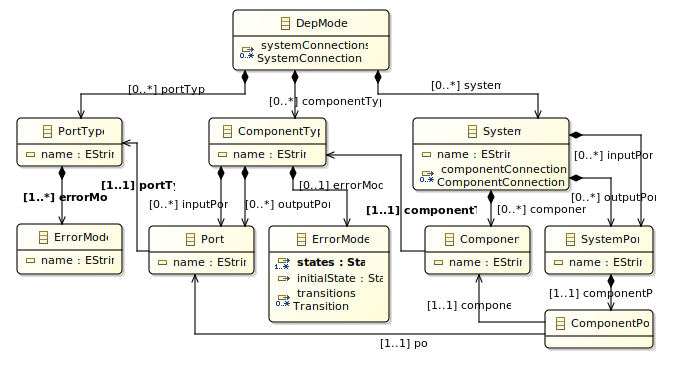
\includegraphics[scale=0.825]{figures/depmodel_metamodel}
  \caption{Architectural modeling language metamodel.}
  \label{fig:architecture:metamodel}
\end{figure}

\begin{figure}
  \centering
  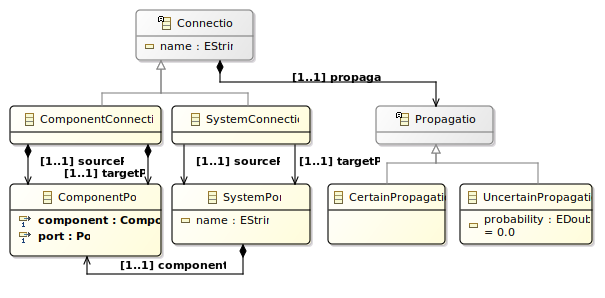
\includegraphics[scale=0.825]{figures/depmodel_metamodel_connections}
  \caption{Connections between ports in the architectural modeling language metamodel.}
  \label{fig:architecture:connections}
\end{figure}

\begin{figure}
  \centering
  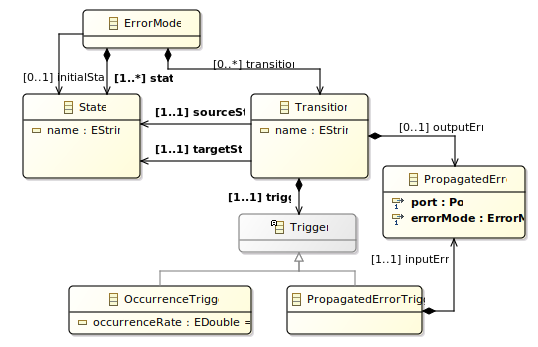
\includegraphics[scale=0.825]{figures/depmodel_metamodel_error}
  \caption{Error models in the architectural modeling language metamodel.}
  \label{fig:architecture:error}
\end{figure}

\Vref{fig:architecture:telecare} shows a portion of the telecare system example architecture by \citet[Chapter~7]{Ecsedi16architecture}. The graphical concrete syntax was created for the language using the Sirius\footnoteurl{http://www.eclipse.org/sirius/} framework as part of our collaboration with the industrial partner.\footnote{Icons used in the graphical syntax are available in the \emph{Fugue Icons} library by Yusuke Kamiyamane under the Creative Commons Attribution 3.0 license at \url{http://p.yusukekamiyamane.com/}}

\begin{figure}
  \centering
  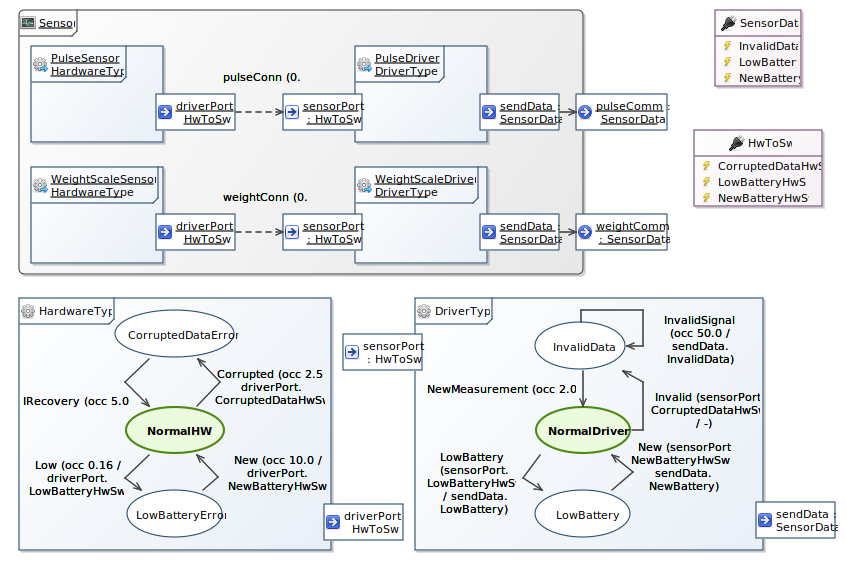
\includegraphics[width=\textwidth]{figures/telecare_system}
  \caption{Telecare system architecture example.}
  \label{fig:architecture:telecare}
\end{figure}

\section{Graph queries}

We implemented the transformation of the architectural modeling language to Petri nets, which was proposed by \citet[Chapter~6]{Ecsedi16architecture}. The transformation allows studying the hazard rates of propagated errors under the assumption that only a single error occurs during system operation per port instance and error mode.

The modeling language contains port types and component types, as well as their instances. Hence it offers some features for multi-level metamodeling. Component instances in systems do not contain individual objects for their ports; furthermore, port instances in component types do not contain individual objects for the error modes of their port instances. Hence ports of component instances must be identified by pairs \(\langle \textit{Component}, \textit{Port} \rangle\), while error modes are identified by triples \(\langle \textit{Component}, \textit{Port}, \textit{ErrorMode} \rangle\). Similar techniques are employed for referencing states and transitions of component instances.

\lstinputlisting[style=block,language=vql,caption={Dependability.vql}]{figures/Dependability.vql}

\section{Petri net modules}

Various Petri net modules were created for the transformation. The module \lit{StateModule} contains a single reference, which will be used to simulate \enquote{rule inheritance} of the \lit{InitialStateModule} and \lit{ErrorStateModule} modules.

The aim of the analysis model is provide hazard rate analysis for port instances of components. Because port instances of component instances are not represented directly as objects in the architectural model, derived features cannot be used for the metrics. We instead bind a \lit{@FaultConfiguration} analysis annotation to a symbol in the \lit{PortModule}, which is instantiated for each port instance of each component instance.

\lstinputlisting[style=block,language=ecore2pn,caption={DependabilityModules.ecore2pn}]{figures/DependabilityModules.ecore2pn}

\section{Transformation specification}

The transformation specification instantiates the \textabbr{RGSPN} modules according to the mapping defined by \citet[Chapter~6]{Ecsedi16architecture}.

States of component instances, as well as the error modes of port instances owned by every component instance are represented as single places. Connecting Petri net fragments describe state transitions and error mode propagation.

\lstinputlisting[style=block,language=ecore2pn,caption={DependabilityPetriNet.ecore2pn}]{figures/DependabilityPetriNet.ecore2pn}